\documentclass{standalone}
\usepackage[dvipsnames]{xcolor}
\usepackage{tikz}
%\usepackage{pgfplots}
%\usepackage{pgfplotstable}
%\pgfplotsset{compat=1.5}
\usetikzlibrary{patterns}
\tikzstyle{v par}=              [dash pattern=on 10pt off 5pt,color=red!70,line width = 2pt]
\tikzstyle{z direction}=      [dash pattern=on 10pt off 5pt on 2pt off 5pt, color=Blue,line width = 2pt]

\begin{document}
{
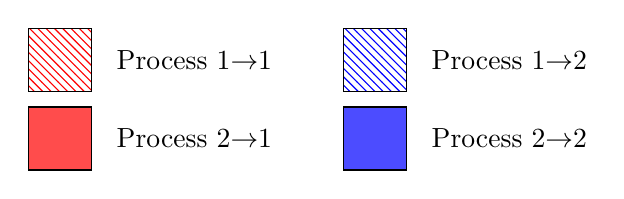
\begin{tikzpicture}
 \begin{scope}[xshift=-4cm]
  \draw[fill=red!70] (0,0) rectangle (0.8,0.8);
  \node[right] at (1,0.4) {Process 2$\rightarrow$1};
  \draw[pattern=north west lines, pattern color=red] (0,1) rectangle (0.8,1.8);
  \node[right] at (1,1.4) {Process 1$\rightarrow$1};
 \end{scope}
  \draw[fill=blue!70] (0,0) rectangle (0.8,0.8);
  \node[right] at (1,0.4) {Process 2$\rightarrow$2};
  \draw[pattern=north west lines, pattern color=blue] (0,1) rectangle (0.8,1.8);
  \node[right] at (1,1.4) {Process 1$\rightarrow$2};
\end{tikzpicture}
}
\end{document}
